\documentclass[12pt]{report}
\usepackage[utf8]{inputenc}
\usepackage[french]{babel}
\usepackage[T1]{fontenc}
\usepackage{amsmath}
\usepackage{amsfonts}
\usepackage{amssymb}
\usepackage{color}
\usepackage{ulem}
\usepackage{graphicx}
\usepackage{titlesec}
\usepackage{caption}
\usepackage{titling}
\usepackage{booktabs}
\usepackage{enumitem}
\usepackage{eurosym}
\usepackage{epigraph}
\usepackage{hyperref}
\usepackage{fontspec}
\usepackage{ragged2e}
\usepackage{parskip}
\usepackage{wrapfig}
\usepackage{calc}
\usepackage{float}

\graphicspath{ {../../static/} {img/} }
\setlength{\droptitle}{-10em}
\titleformat{\chapter}[hang]{\normalfont\huge\bfseries}{\thechapter. }{0em}{}

\begin{document}

\title{
	{\vspace{3em}\protect\centering\protect
\includegraphics[width=0.9\textwidth]{Pacification_logo}}\\
	{\vspace{4em}\Huge Rapport de projet}\\
	{\large Brainless Devs}
}
\author{
	Thibault Allançon\\
	Valérian Fayt
	\and
	Antoine Gonzalez\\
	Cédric Parpet}
\date{
	{\vfill\protect\centering\protect
\includegraphics{brainless_devs.pdf}}\\
	Dossier Projet Informatique\\
	Info-Sup EPITA\\
	Mai 2018
}

\maketitle
\tableofcontents

\chapter{Remerciements}

Nous souhaiterions remercier Jasper Flick pour ses articles C\#/Unity d'une
excellente qualité (\url{https://catlikecoding.com/}), Michsky pour son asset de
menu mis à notre disposition, ainsi que le site \url{www.mixamo.com} qui nous a
permi d’obtenir des animations pour nos personnages.

Enfin nous voudrions remercier profondément toutes les personnes qui nous ont
aidés au cours du développement de notre jeu, que ce soit au niveau de conseils
ou en testant le jeu pour nous faire remonter les problèmes et incohérences.
Merci à Théo Versaille, Nassim Fortas, Lucas Ligny, Nicolas Cantaert, Cindy
Delebecque, Kenny Lorin et bien d'autres !

\chapter{Introduction}

C’est 5 mois après le début de son développement que nous concluons la création
de Pacification, notre jeu vidéo de stratégie se basant sur l’univers des jeux
Civilization. Acceptant jusqu'à 8 joueurs simultanément, Pacification mettra vos
stratégies à l’épreuve pour combattre tant d’ennemis. Un mode solo vous
permettra aussi d’apprendre à maîtriser le jeu, et un éditeur vous offrira la
possibilité de personnaliser votre expérience de jeu en créant vos propres
territoires de batailles.

Il s’agit d’un projet ambitieux que nous avons pu mener à terme, mêlant nos
compétences et nos expériences. Ayant réalisé par nous même l’intégralité des
modèles 3D et textures du jeu, nous sommes fiers du rendu final de ce projet
auquel nous avons dédié beaucoup de temps.

Ce rapport aura pour objectif de vous présenter un compte-rendu de tout ce
semestre, avec les évolutions au cours du temps et l'accomplissement des
objectifs, de même que la répartition des tâches au sein du groupe.

\chapter{Généralités}

\section{Inspiration}

Dans un premier temps, nous hésitions entre réaliser un jeu de stratégie ou de
plateforme-réflexion. Après discussions et quelques consommations de pizza nous
avons opté pour le jeu de stratégie. Plusieurs réunions nous ont permis de fixer
les prémices du jeu, ainsi que les fonctionnalités voulues.

Pacification prend son inspiration dans divers jeux stratégiques cultes tels que
Age of Empire mais aussi particulièrement Civilization. En effet, notre jeu
ressemble aux jeux type 4X (eXplore, eXpand, eXploit, eXterminate) dont le
premier représentant a été Empire (1977) et dont d’autres exemples sont très
connus (la série Civilization, Master of Orion). Ces jeux ont des codes
spécifiques comme la construction d’un empire, un gameplay au tour par tour, la
gestion de leur économie, des améliorations technologiques, une vue de haut et
globale sur la carte du monde. 

Avec cet objectif en tête, il s’agissait alors de déterminer le nom  du jeu
auquel nous allions donner vie. Cette partie fut sans conteste la plus longue de
notre première réunion. L’objectif étant de combiner une appellation à la fois
humoristique et originale, d’où l’ironie de “Pacification” puisque l’une des
occupations principales du jeu est de « pacifier les tribus barbares », car
comme disait Montaigne, « chacun appelle barbarie ce qui n’est pas de son usage
».

\section{Déroulement d’une partie}

Le joueur commence la partie sur une carte générée aléatoirement selon des
paramètres choisis par lui-même. Il dispose alors d’un colon et d’un fantassin.
Le colon va lui permettre de construire sa première ville, tandis que le
fantassin va pouvoir entamer l’exploration des environs et défendre le colon. Le
joueur va devoir mettre au point une stratégie et apprendre à gérer ses
ressources afin de réagir à l’évolution de la partie et remporter la victoire
face à ses adversaires. Il lui faudra explorer la carte, développer son armée,
exploiter les ressources disponibles et utiliser le terrain à son avantage pour
en ressortir vainqueur.

En solo, le joueur devra faire face à une IA et résister aux assauts fréquents
des barbares afin d’atteindre le dernier niveau technologique pour réaliser une
victoire scientifique.

En multijoueur, les joueurs s’affronteront jusqu’à ce qu’il n’en reste qu’un,
plus aucunes unités ou villes ennemies ne doit rester debout.

\section{Logiciels utilisés}

Pour réaliser ce projet nous avons utilisé le moteur de jeu Unity, l’avantage
étant qu’il s’agit d’un moteur puissant, complet et grandement documenté. Ceci
nous a permi de réaliser un jeu en 3D stable avec un multijoueur en un temps
raisonnable. Unity supporte le scripting en C\#, un langage de programmation
orienté objet développé par Microsoft, que nous avons utilisé tout au long du
projet. Le paradigme orienté objet est un choix indispensable pour maintenir un
projet aussi conséquent, afin de profiter des avantages de l’encapsulation, de
l’héritage, ainsi que du polymorphisme.

Le second logiciel qui a été nécessaire à la réalisation de nos assets, est
Blender. Un logiciel de modélisation, d’animation et de rendu 3D très populaire
et gratuit.

Enfin, nous n’aurions pu mener ce projet à bien sans Git, un gestionnaire de
version, ainsi que GitHub pour l'hébergement du dépôt du projet.

\chapter{Le groupe}

\section{Présentation de l'équipe}

\begin{itemize}[label=\textbullet]
    \item \textbf{Thibault Allançon (Chef de projet)} : Prophète GNU/Linux,
        venant apporter la bonne nouvelle et convertir les hérétiques vers le
        Saint OS. Gourou algorithmicien et dictateur durant son temps libre, il
        a su diriger ce projet \textbf{fermement} (à l’aide de violence verbale
        et physique, enfin c’est ce que disent les rumeurs).
    \item \textbf{Cédric Parpet} : Amateur de jeu de stratégie tel que la série
        des \textit{Age of empire}, \textit{Mythologie} et \textit{Warcraft}, il
        a déjà codé les bases d’un jeu de stratégie au tour par tour pour son
        projet d’ISN. La légende dit qu’il code avec ses longs cheveux qui sont
        par ailleurs très soyeux (c’est de la fibre, à seulement
        19\euro99/mois).
    \item \textbf{Valérian Fayt} : Il s’est découvert une passion pour les jeux
        de stratégie bien jeune et y a sans doutes passé trop de temps. Tout
        comme son voisin aux longs cheveux, il a lui aussi grandement apprécié
        la série des \textit{Age of Empire}. Peu expérimenté au codage en début
        d'année, ce projet a été l'occasion pour lui d'apprendre beaucoup et
        repousser ses limites. Vers l’infini et l’au-delà !
    \item \textbf{Antoine Gonzalez} : Il vit en France, mais son fuseau horaire
        est incertain. Parfois il hiberne pendant des jours entiers. Parfois il
        code non-stop. Parfois il apprend quelque chose de nouveau, because why
        not. Sinon, il contemple le sens de son existence, entre deux ragequit
        (on le surnomme le Pape Salé). Mais il s’éloigne rarement de
        l’ordinateur, sauf pour s’alimenter, éventuellement. Il a plus de
        respect pour les CGU que pour son fournisseur internet.
\end{itemize}

\section{Répartition des tâches}

Seulement deux changements mineurs pour les rôles, après la première soutenance
nous nous sommes rendu compte que les assets demanderaient énormément de temps
et que l'interface serait une partie importante du jeu, Antoine et Valérian sont
donc passés suppléants UI afin d'aider Cédric.

\vspace{0.5cm}

\begin{center}
    \begin{tabular}{@{} l *4c @{}}
        \toprule
        \multicolumn{1}{c}{}    & \textbf{Thibault}  & \textbf{Antoine}  & \textbf{Cédric} & \textbf{Valérian} \\ 
        \midrule
        Map & R & S & & \\
        IA & R & & & \\
        Réseau & & S & S & R \\
        Graphisme & & & R & \\
        UI & & \underline{\textbf S} & R & \underline{\textbf S} \\
        Site web & & & & R \\
        Gameplay & S & R & & S\\
        \bottomrule
        \multicolumn{4}{l}{\footnotesize R = responsable, S = suppléant}\\
    \end{tabular}
\end{center}

\section{Objectifs des soutenances}

Plannifier autant de tâches à l'avance n'était pas évident, cependant nos
estimations étaient plutôt bonnes et nous avons su nous y tenir jusqu'au bout.

\begin{center}
    \begin{tabular}{@{} l *4c @{}}
        \toprule
        \multicolumn{1}{c}{}    & \textbf{Soutenance 1}  & \textbf{Soutenance 2}  & \textbf{Soutenance 3} \\ 
        \midrule
        Map & 65\% & 100\% & 100\% \\
        IA & \sout{30} {\color{red} 20}\% & 70\% & 100\% \\
        Réseau & \sout{30} {\color{green} 50}\% & \sout{75} {\color{green} 85}\% & 100\% \\
        Assets & \sout{50} {\color{red} 40}\% & 100\% & 100\% \\
        Interface & 10\% & \sout{80} {\color{red} 70}\% & 100\% \\
        Site & \sout{10} {\color{green} 60}\% & 95\% & 100\% \\
        Gameplay & 40\% & 80\% & 100\% \\
        Budget pizza & 100\% & 60\% & null\\
        \midrule
        Jouabilité & 25\% & 60\% & 100\% \\
        \bottomrule
    \end{tabular}
\end{center}

Avec un jeu qui a rapidement pris forme, cela nous a motivé à travailler
davantage dessus et à rajouter plusieurs composantes en plus de celles déjà
présentes :

\begin{itemize}
    \item Un tchat en multijoueur pour communiquer avec les autres
    \item Un éditeur de carte
    \item La possibilité d'embarquer sur l'eau et se déplacer sur les océans
    \item Une gestion du son avec des musiques d'ambiancce ainsi que quelques
        bruitages
    \item Différentes animations (mouvement, attaque, mort)
    \item Quelques effets de particules
\end{itemize}

\chapter{Le jeu}

\section{Map (Thibault)}

\subsection{Construction}

La particularité de la carte est qu’elle est entièrement constituée d’hexagones.
Ceci nécessitait une certaine réflexion pour anticiper différents aspects comme
le rendu graphique, le pavage, les relations entre les multiples voisins, ou
encore le système de coordonnées des cases.

\begin{figure}
    \centering
    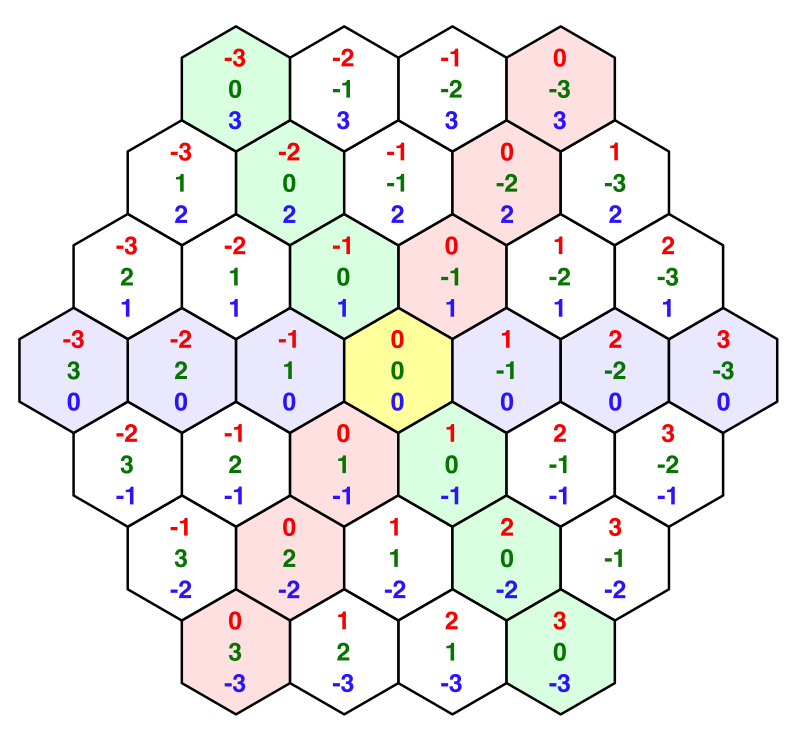
\includegraphics[width=0.5\textwidth]{../report_1/img/cubic_coordinates}
    \caption*{Système de coordonées et axes}
\end{figure}

Pour supporter de grandes tailles de carte ainsi qu’un mode multijoueur
accueillant jusqu’à 8 joueurs, il fallait découper la carte en chunks pour
éviter d’avoir un unique mesh gigantesque à actualiser constamment. Le rendu
graphique est alors considérablement allégé.

Plusieurs modifications sont possibles sur la carte :

\begin{itemize}
    \item Définir des biomes (ce qui change les textures du terrain)
    \item Créer des montagnes d’une hauteur variable
    \item Possibilité de relier des cases entre elles à l’aide de routes
    \item Rajouter de l’eau pour constituer des océans
    \item Placer des ressources (fer, or, diamant, chevaux, etc.) ou des
        constructions (ferme, exploitation arboricole, ville, etc.)
\end{itemize}

\begin{figure}
    \centering
    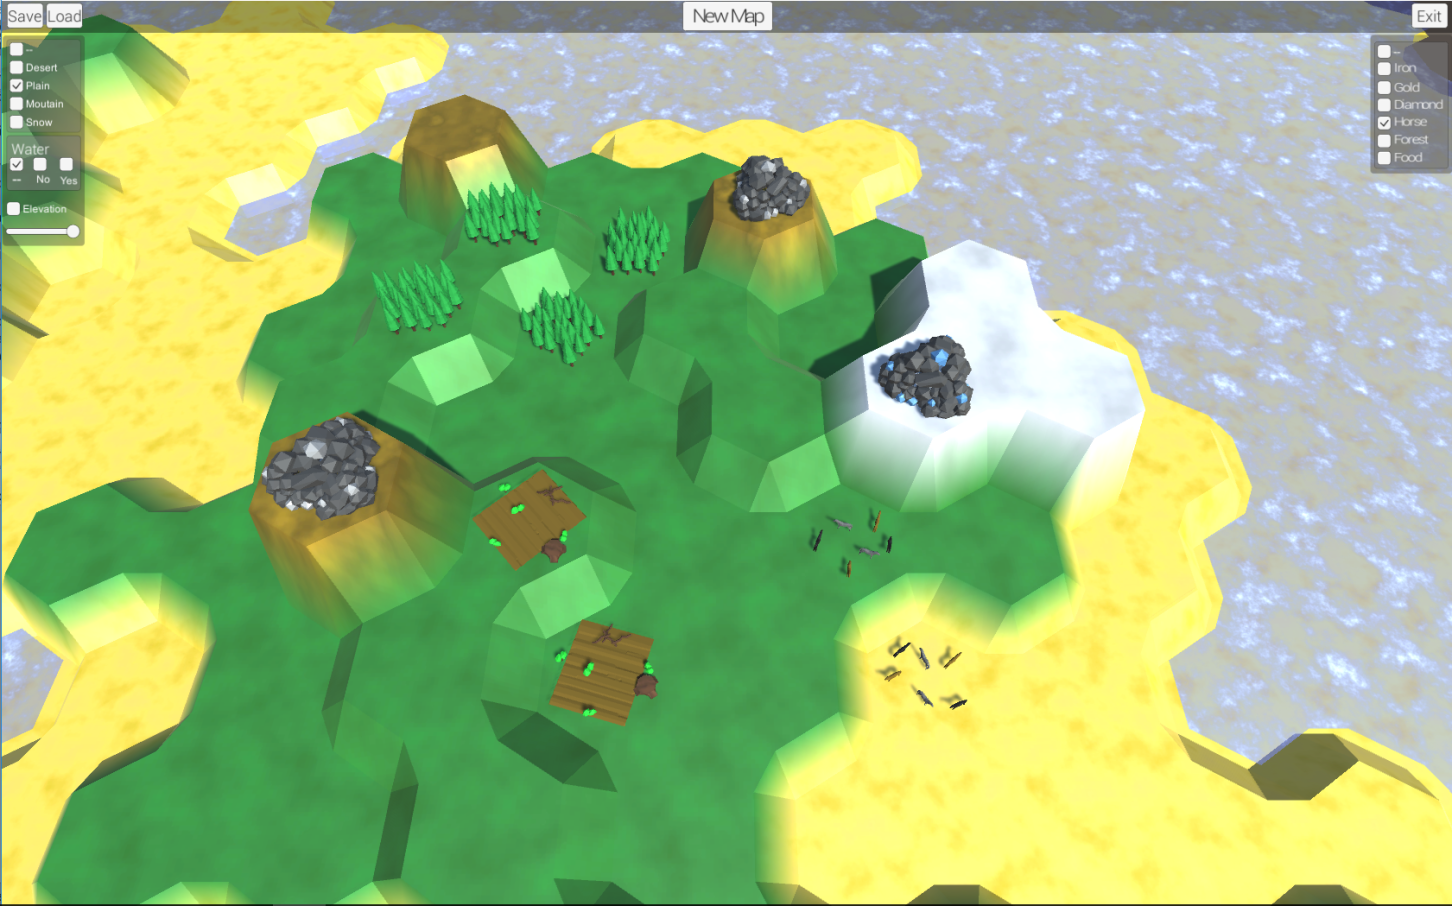
\includegraphics[width=0.9\textwidth]{map_example}
    \caption*{Exemple de carte de jeu dans l'éditeur}
\end{figure}

\subsection{Brouillard de guerre}

Un élément fondamental pour un jeu de stratégie était un système de brouillard
de guerre. Le mettre en place fût plus compliqué que prévu, car une gestion
précise des shaders ainsi que des textures n’est pas une tâche facile à
accomplir. De plus il a fallu ajouter aux unités un système de vision qui prend
en compte l’environnement ainsi que les caractéristiques de l’unité en question.

On distingue deux types de brouillard :

\begin{itemize}
    \item Les cases totalement inexplorées par le joueur qui sont entièrement
        grisées
    \item Les cases précédemment explorées, mais hors de vision des
        unités/villes du joueur, qui sont légèrement noircies.
\end{itemize}

\begin{figure}
    \centering
    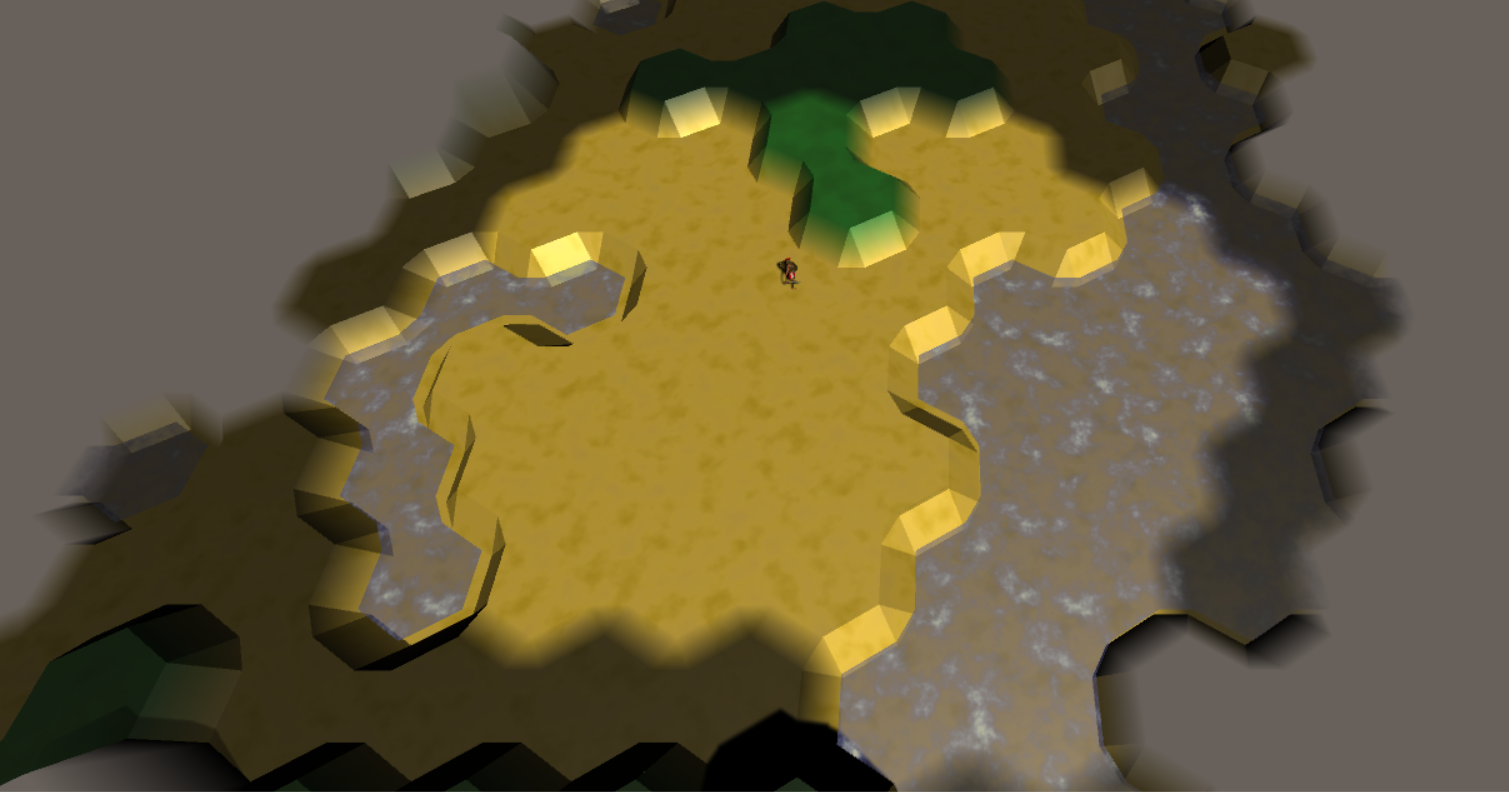
\includegraphics[width=0.8\textwidth]{../report_2/img/FogOfWar}
    \caption*{Brouillard de guerre}
\end{figure}

\subsection{Génération procédurale}

Après la première soutenance où nous montrions les différentes modifications
possibles de la carte, nous avons décidé de transformer cette partie du code
pour créer un éditeur de carte. Cependant, il était convenu depuis le début
qu’une génération procédurale permettrait au joueur d’avoir un environnement
différent à chaque partie.

Cette génération est constituée d’une dizaine de paramètres modifiables comme le
pourcentage de terre, le niveau d’érosion des terrains, le nombre/taille des
régions, l’élévation maximale des montagnes, etc. Pour créer une nouvelle carte,
il faut décider des parties du terrain qui vont être surélevées (toute la carte
est à la base un océan géant entièrement plat). Une gestion de l’aléatoire était
fondamentale pour cette partie de la carte, et le joueur peut utiliser des
“seed” afin d’initialiser ce générateur pseudo-aléatoire. Une fois la case (qui
servira de point de départ d’une région) choisie, un parcours en largeur permet
de surélever les environs en conserver cet aspect de région. Les biomes des
cases sont attribuées à la fin, en fonction de l’élévation du terrain (par
exemple le terrain de très basse altitude sera une plaine ou un désert, mais un
terrain en hauteur sera soit une simple montagne rocheuse, soit une montagne
enneigée).

\begin{figure}[H]
    \centering
    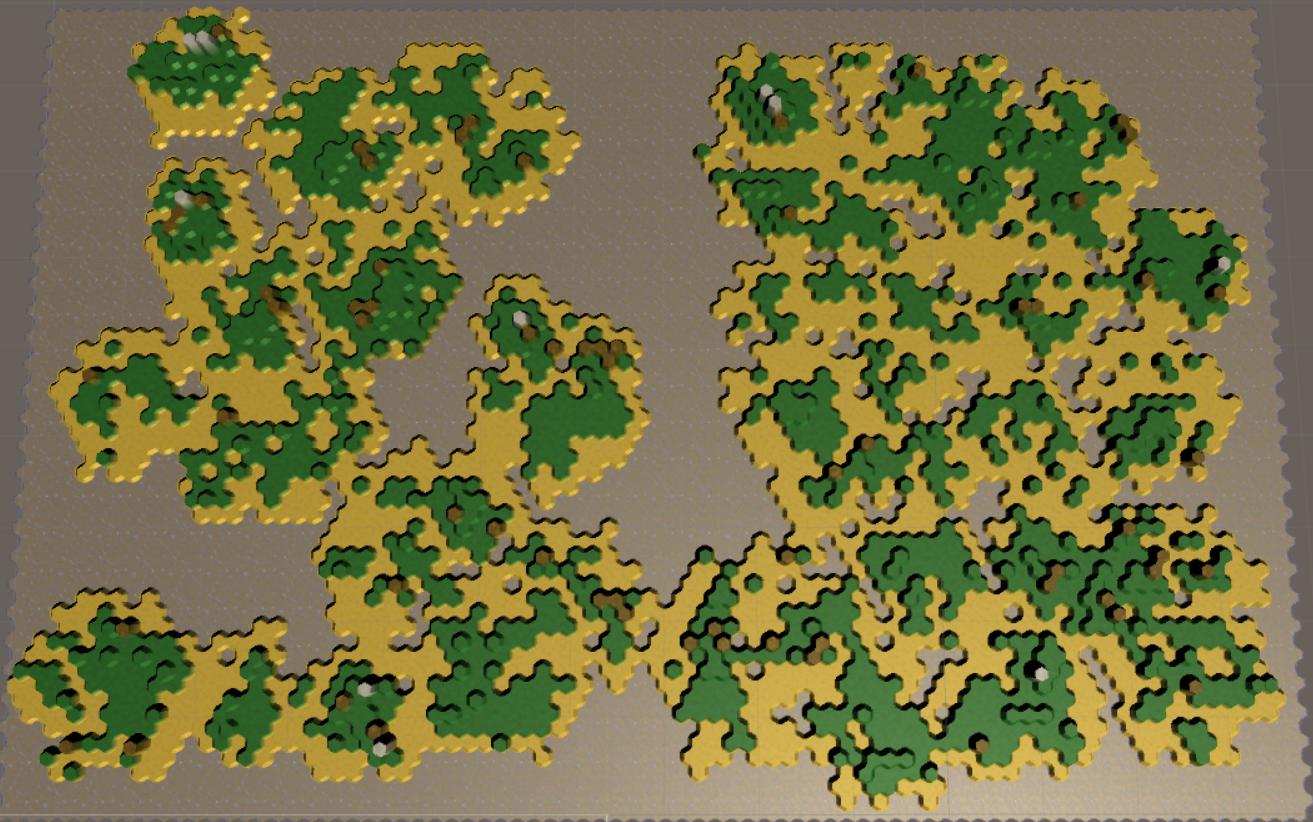
\includegraphics[width=0.8\textwidth]{../report_2/img/MapGen1}
    \caption*{Génération de carte 1}
\end{figure}

\begin{figure}[H]
    \centering
    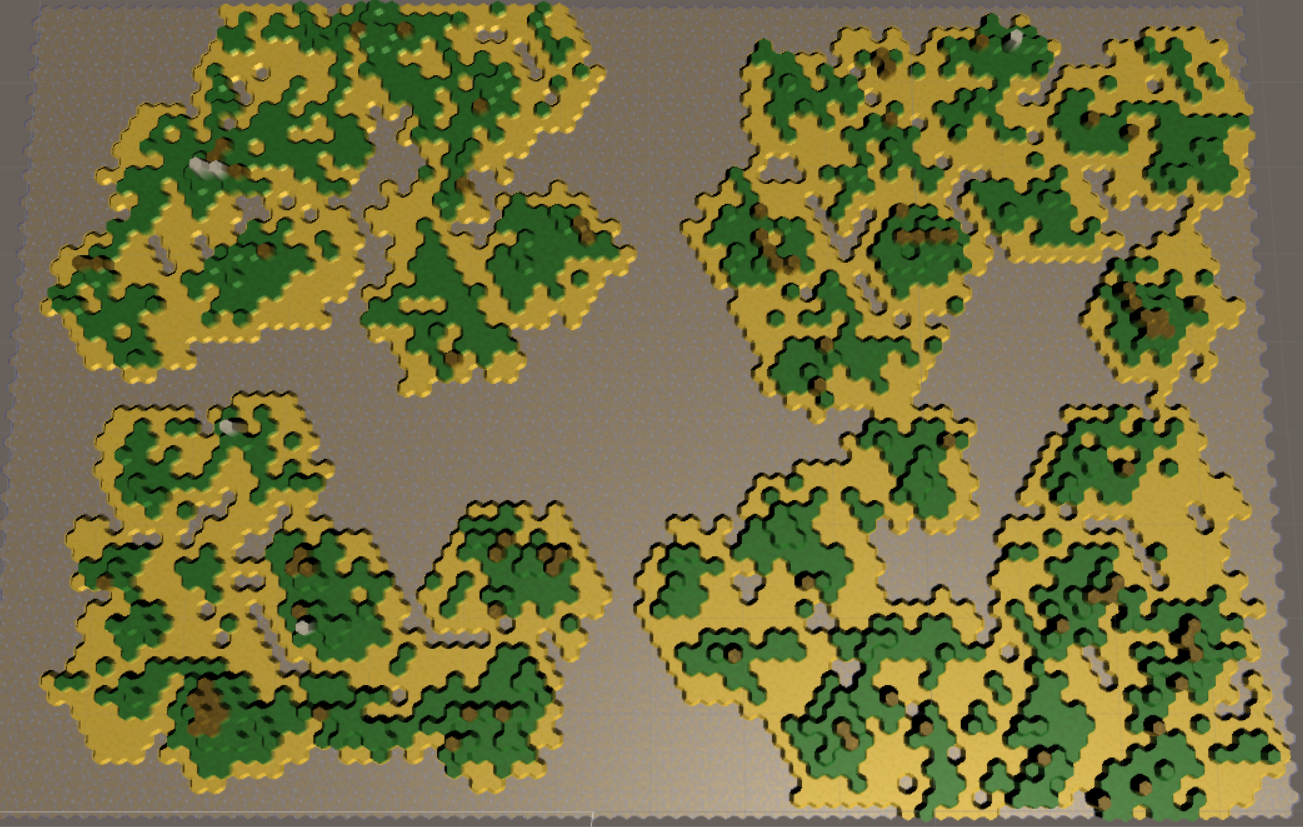
\includegraphics[width=0.8\textwidth]{../report_2/img/MapGen2}
    \caption*{Génération de carte 2}
\end{figure}

Les ressources sont placées aléatoirement autour des points de départ des
joueurs à la fin de la génération, et sont dispersés sur le reste de la carte
en fonction notamment des biomes.

\subsection{Interactions}

\subsubsection{Utilisateur}

Côté utilisateur, il était nécessaire d’avoir une gestion correcte de la caméra
ainsi que des contrôles (comme le clic ou les raccourcis clavier). Il y a donc
une possibilité de déplacer, zoomer avec la caméra, de sélectionner une
case/unité/ville, de faire des actions à l’aide de touches (attaquer, créer une
route, fonder une ville). La caméra peut aussi se focaliser sur un endroit
précis de la carte, permettant au joueur de passer rapidement d’une unité à une
autre, ou d’une ville à une autre avec des raccourcis.

\begin{figure}[H]
    \centering
    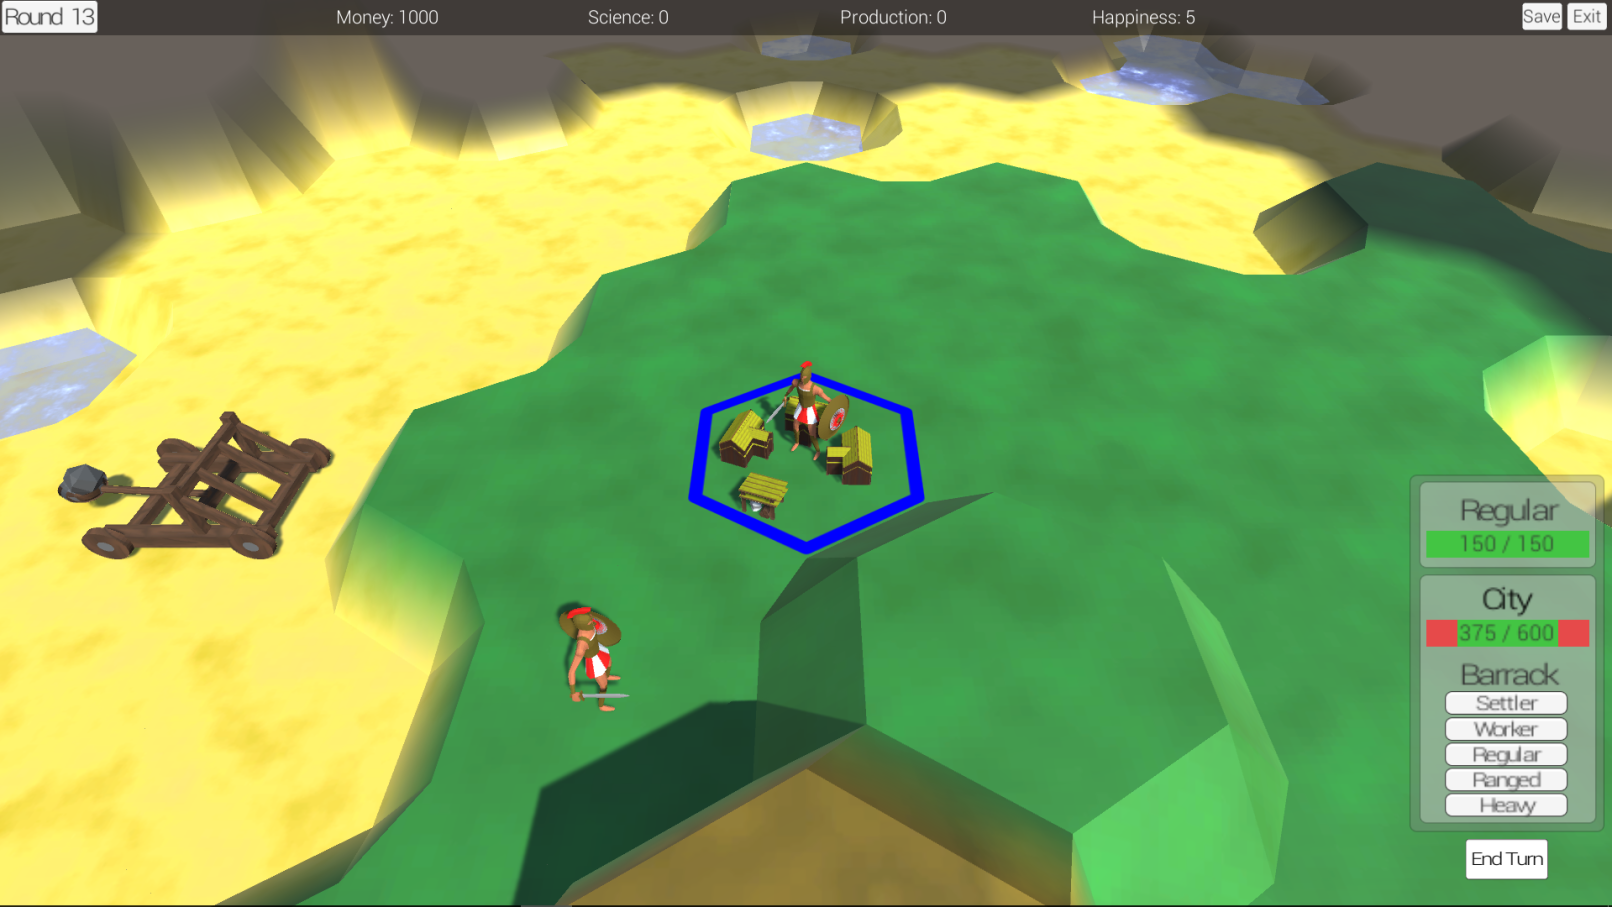
\includegraphics[width=0.8\textwidth]{game_ui}
    \caption*{L'interface utilisateur}
\end{figure}

\subsubsection{Unités}

L’interaction la plus importante concernant la carte est celle du déplacement
des unités. Il faut gérer d’une part la recherche du plus court chemin sur la
carte à l’aide de l’algorithme A*, prenant en compte de nombreuses
caractéristiques comme la vitesse de déplacement des unités, les obstacles, ou
encore les spécificités des biomes.

\begin{figure}[H]
    \centering
    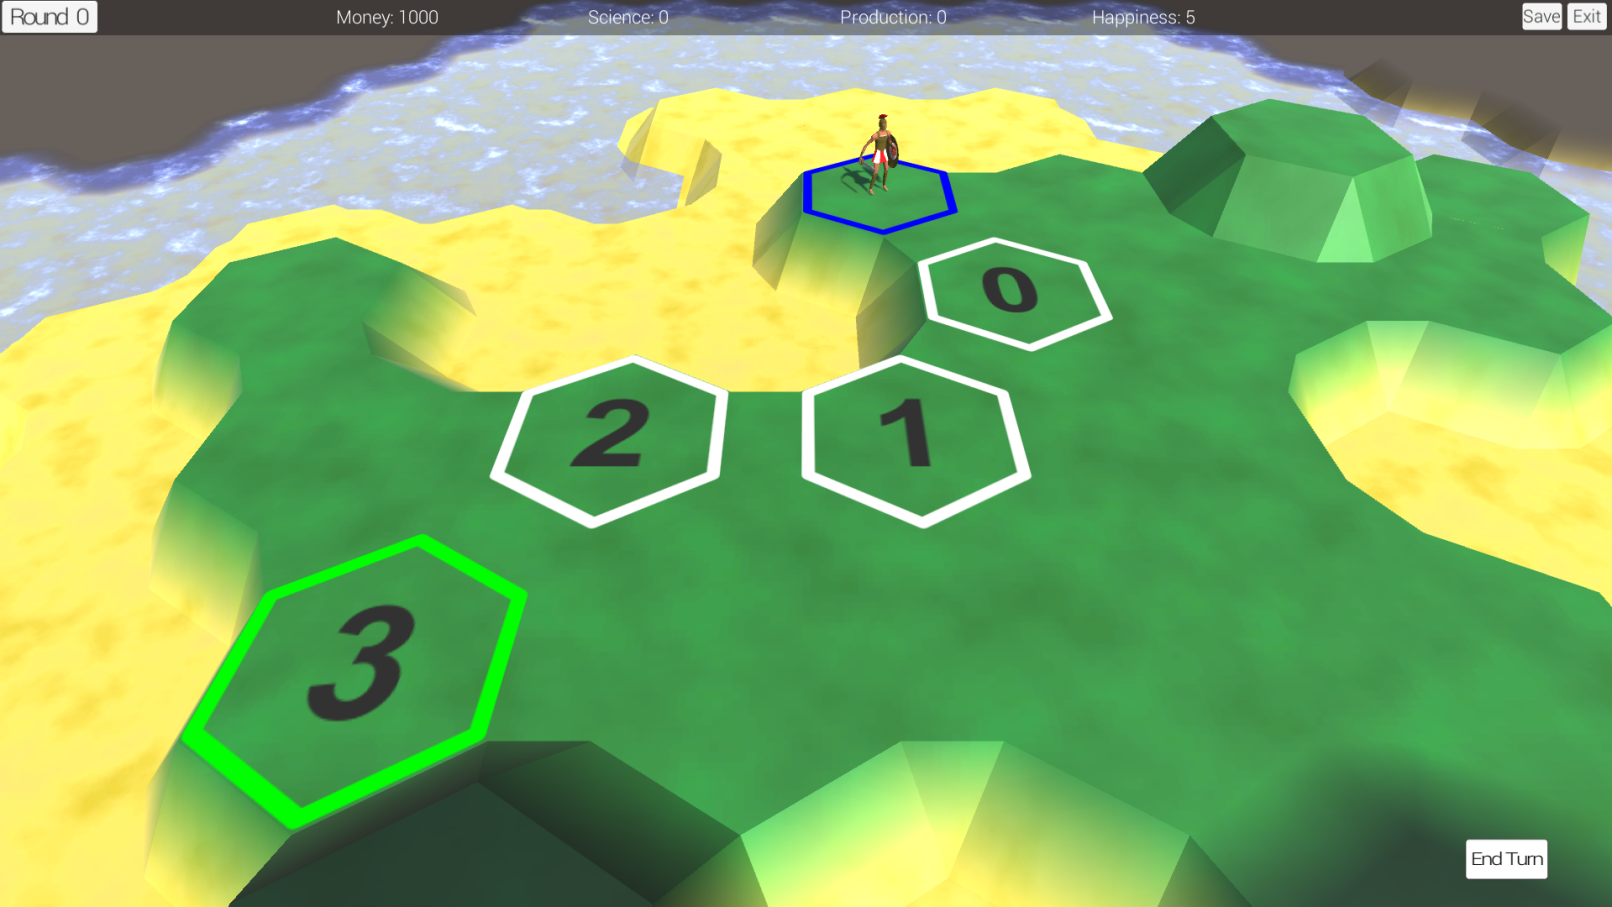
\includegraphics[width=0.3\textwidth]{pathfinding1}
    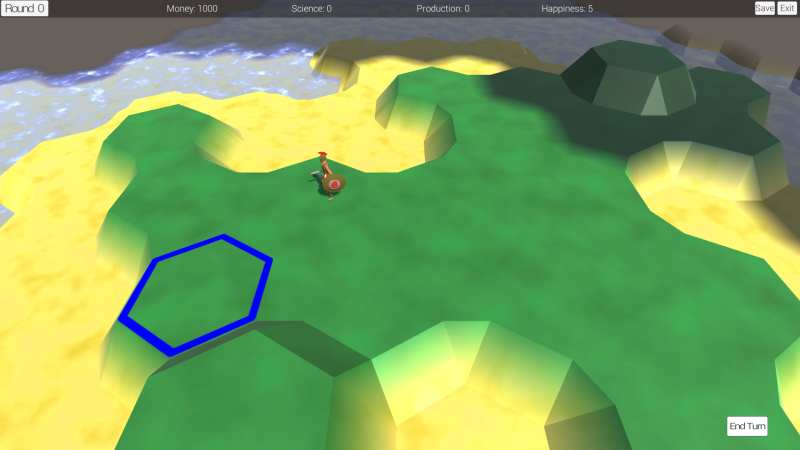
\includegraphics[width=0.3\textwidth]{pathfinding2}
    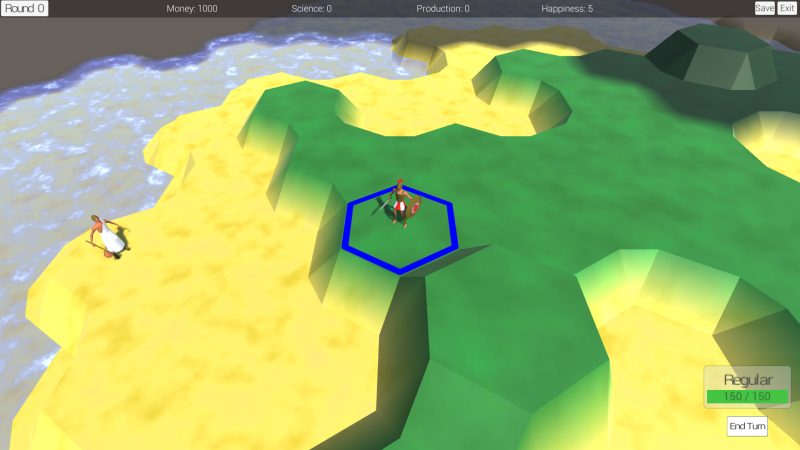
\includegraphics[width=0.3\textwidth]{pathfinding3}
    \caption*{Déplacement d'une unité}
\end{figure}

De plus, l’affichage du chemin est primordial pour le joueur, ainsi que les
animations de mouvement. Des courbes de Bézier sont utilisées pour simuler des
déplacements fluides et plus naturels, ainsi que l’orientation des unités durant
leurs déplacements d’une case à une autre.

Chaque unité possède une action principale :

\begin{itemize}
    \item Pour le colon : fonder une ville
    \item Pour l’ouvrier : exploiter une case
    \item Pour l’attaquant : attaquer une unité/ville
\end{itemize}

L’ouvrier possède une deuxième action qui est de construire une route entre deux
cases. Cette partie fût relativement compliquée à mettre en place, pour gérer
correctement les multiples voisins d’un hexagone, ainsi que la triangulation
pour l’aspect graphique.

\begin{figure}[H]
    \centering
    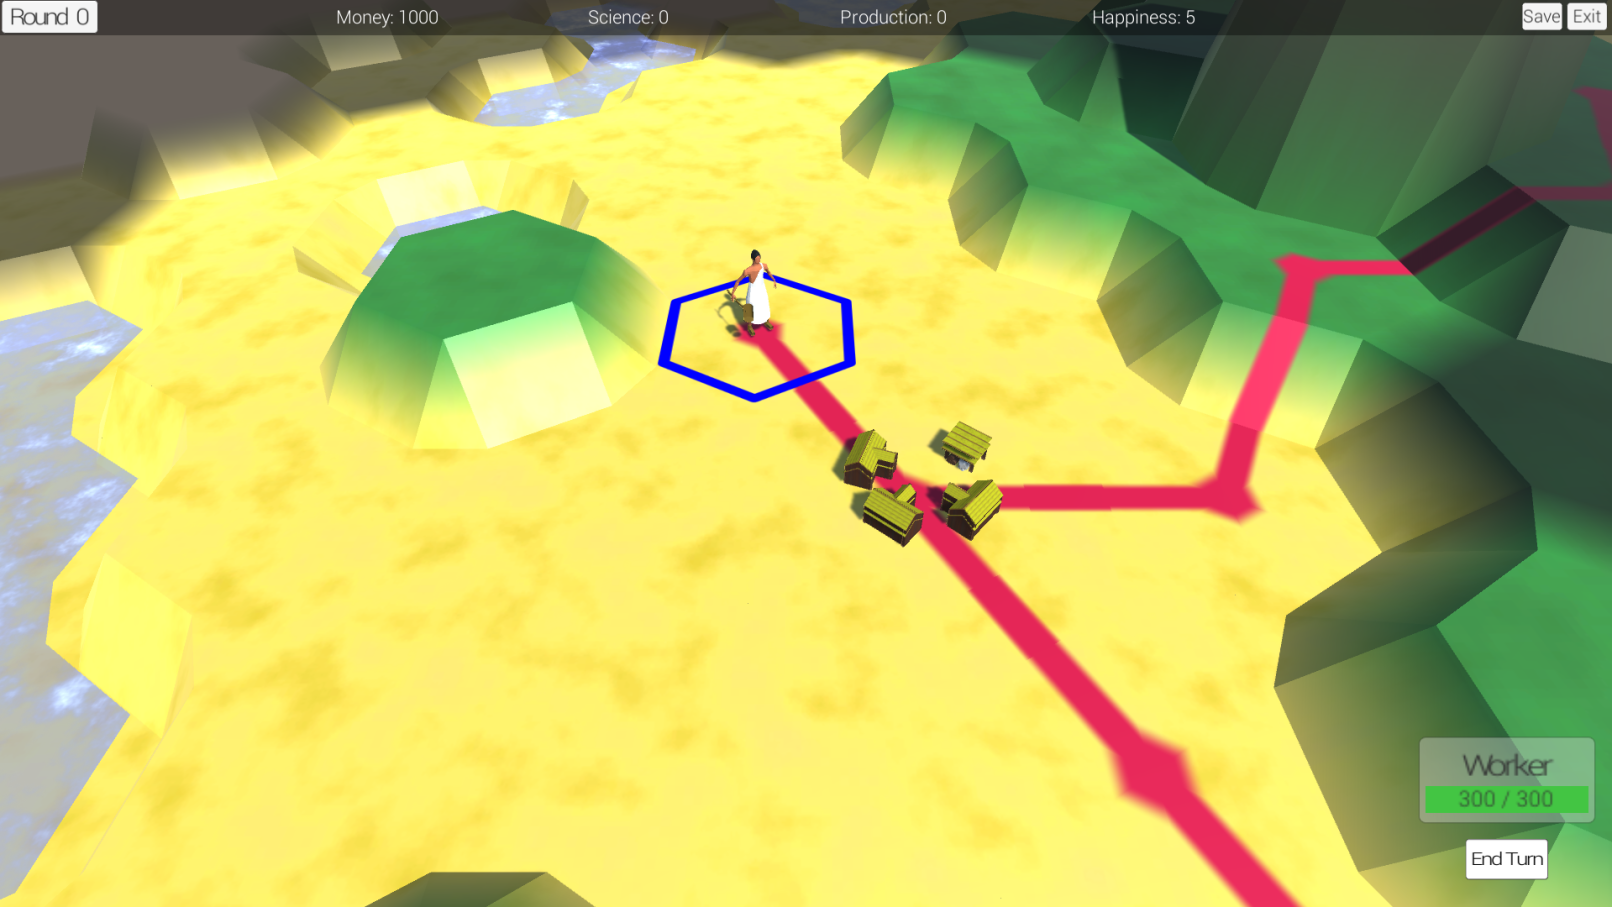
\includegraphics[width=0.8\textwidth]{worker_road}
    \caption*{Une construction de route par l'ouvrier}
\end{figure}

À partir d'un certain niveau technologique, toutes les unités ont la
possibilité d'embarquer sur l'eau pour traverser les océans.

\begin{figure}[H]
    \centering
    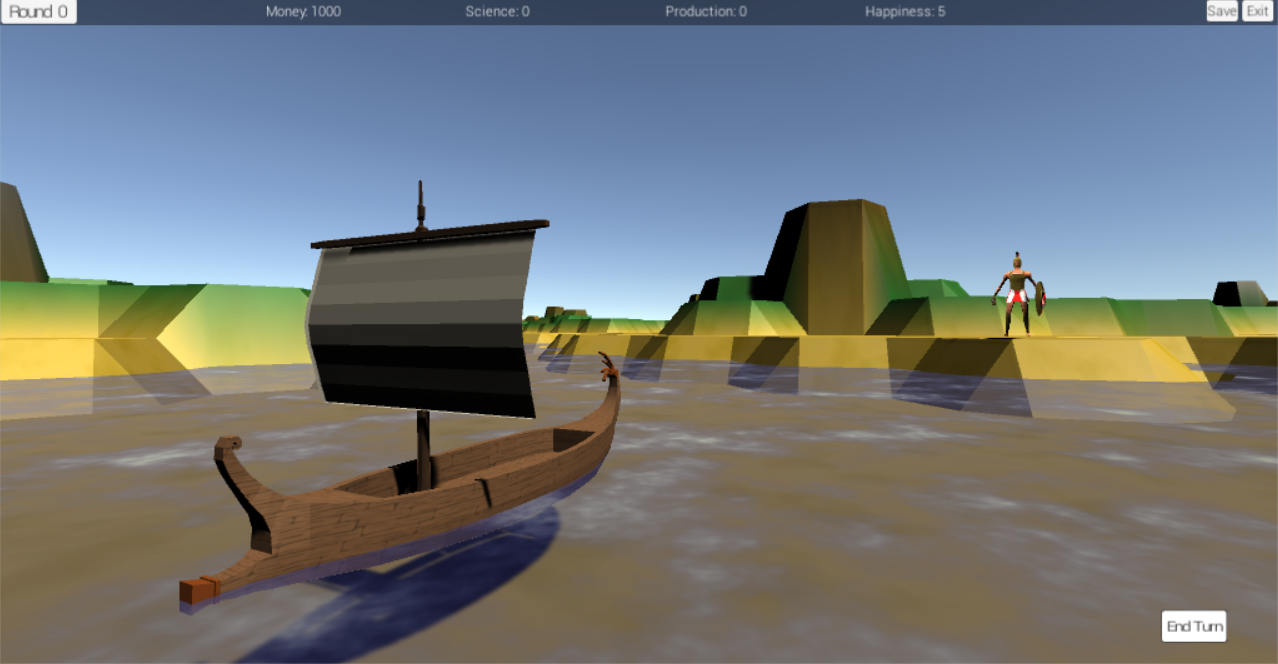
\includegraphics[width=0.8\textwidth]{boat}
    \caption*{Une unité embarquée}
\end{figure}

\subsection{Sauvegarder/Charger une carte}

Sauvegarder et charger des cartes étaient évidemment une nécessité, d’une part
pour l’éditeur de carte afin de jouer avec ses propres créations, mais aussi
pour sauvegarder une partie en cours pour le mode solo afin de pouvoir la
reprendre plus tard.

\section{Réseau et multijoueur (Valérian)}

\subsection{Construction}

Le multijoueur étant le mode de jeu principal de notre projet, son
implémentation a été prioritaire. Pour cette raison, nous nous sommes concentrés
dessus dès le début du projet, et avons travaillé sur ce dernier tout au long
des soutenances.

Pour le rendre fonctionnel, il était nécessaire de posséder une couche réseau
solide afin de relier les différents joueurs ensembles. S’il a d’abord été
envisagé d’utiliser le module réseau proposé par Unity, U-net, nous nous sommes
rapidement rendus compte qu’il ne répondait pas à nos attentes. Ce module ne
nous permettait pas d’avoir un contrôle total sur le réseau du jeu et ne
respectait pas notre envie de fabriquer un maximum d’éléments du jeu par nos
propres moyens. 

C’est pourquoi nous avons développé notre propre infrastructure réseau,
modulable selon nos besoins, et la perspective d’apprentissage étant davantage
intéressante ainsi.

Codé à l’aide des Sockets du C\#, notre couche réseau s’est révélée
fonctionnelle et pratique pour le reste du jeu.

\subsection{Fonctionnement}

Concernant le fonctionnement de ce système, il se base sur un serveur et des
clients qui s’y connectent. Les clients sont activés sur tous les ordinateurs
lorsque ceux-ci tentent de rejoindre une partie. Seul l’hôte de partie dispose
du serveur.

Lorsque le serveur est démarré, il écoute en attendant des connexions de
clients. L’attente dure tant que le lobby de la partie n’est pas rempli (jusqu’à
8 joueurs) ou que la partie n’est pas démarrée manuellement par l’hôte. Les
clients se connectent à ce serveur à l’aide de l’adresse IP de l’hôte. À chaque
tentative de connexion le serveur demande au client de s’identifier, une fois
l’identification terminée, cette dernière est transmise aux autres clients. En
cas de déconnexion, l’information est partagée aux clients encore en ligne. Ce
processus permet à tous les joueurs de savoir à tout moment qui est connecté
dans la partie.

\begin{figure}[H]
    \centering
    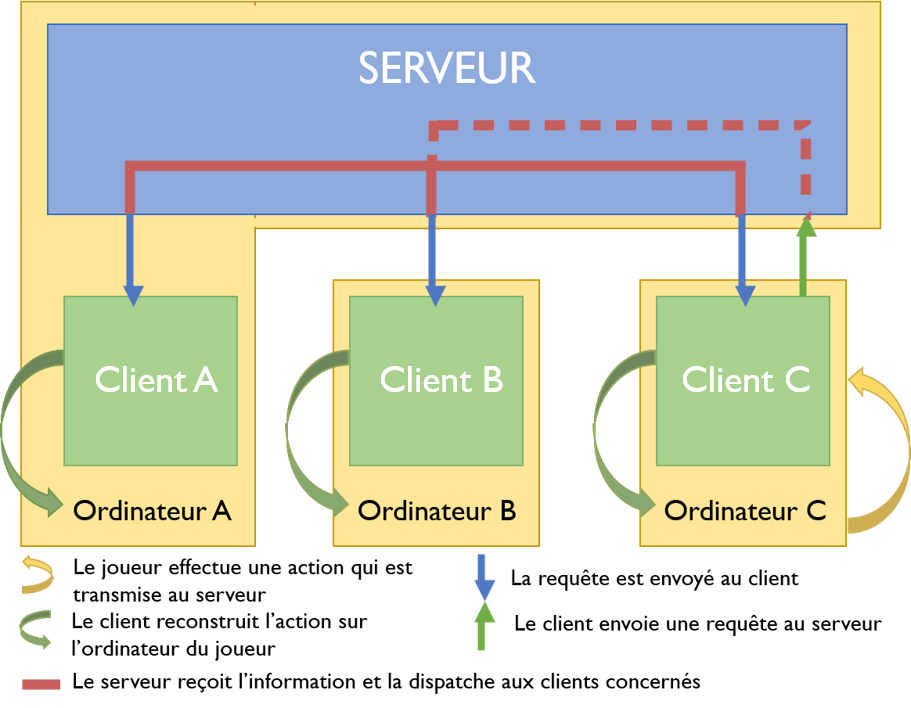
\includegraphics[width=0.8\textwidth]{../report_1/img/multiplayer}
    \caption*{Schéma fonctionnel du réseau}
\end{figure}

Il est possible pour l’hôte de démarrer la partie à partir du moment où 2
joueurs ou plus sont connectés au lobby. Quand la partie est démarrée, le
serveur n’accepte plus de connexion et transmet aux clients un message annonçant
le début de la partie, ce qui lance le jeu sur les ordinateurs de tous les
joueurs. C’est ensuite à la carte de jeu d’être transmise, suivant le processus
détaillé ci-dessus.

\subsection{Principe}

Pendant le jeu, les échanges sont effectués via un processus de sérialisation.
Lorsqu’un joueur effectue une action, celle-ci est sérialisée sous forme de
chaîne de caractères, puis envoyée au serveur qui se charge de dispatcher
correctement le-dit message aux autres joueurs. À la réception d’un message, le
client va reproduire l’action que ce message décrit. Le type d’action est défini
par les quatres premiers caractères du message transmis : 

\begin{itemize}
    \item Le premier caractère indique le type de l’expéditeur (S pour le
        serveur, C pour un client) 
    \item Les 3 suivants indiquent le type d’action, suivant le tableau
        ci-dessous.
\end{itemize}

\vspace{0.5cm}

\begin{center}
	\begin{tabular}{c|c}
		\toprule
		\textbf{Caractères}  & \textbf{Action}\\ 
		\midrule
		WHO & Demande d’identification \\
		IAM & Réponse d'identification \\
		CNN & Nouvelle connexion \\
		DEC & Déconnexion d’un client \\
        KIK & Déconnexion manuelle d’un client \\
        LOD & Lancement de la partie \\
		MAP & Transmission de la map \\
        \\
		END & Annonce de la fin d’un tour \\
		YGO & Autorisation de début de tour\\
        YOP & Autorisation cheat mode\\
        \\
		MOV & Mouvement d’une unité\\
        UNC & Création d'une unité\\
        UTD & Prise de dégâts d'une unité\\
        UNL & Amélioration d'une unité\\
        \\
        WEX & Exploitation de ressources\\
        WRD & Création d'une route\\
        \\
        CLS & Retire toutes les unités de la carte\\
        CIT & Création d'une ville\\
        CID & Destruction d'une ville\\
        CTD & Prise de dégâts d'une ville\\
        \\
        DED & Mort d'un joueur\\
        KIL & Mort manuelle d'un joueur\\
        \\
		MSG & Message global\\
		MSP & Message privé\\
		MSE & Erreur de destinataire du message\\
		\bottomrule
	\end{tabular}
\end{center}

Ce système a ainsi permis la mise en place d’un suivi de l’état des clients
(connecté / déconnecté) synchronisé sur tous les appareils, ainsi qu’un système
de tchat entre les joueurs (public et privé) mais aussi plus particulièrement la
synchronisation du jeu pour les joueurs.

Toute latence de quelques millisecondes qui pourrait survenir avec ce système
n’est pas un problème dans le cas de ce projet, car il ne s’agit pas d’un jeu
nécessitant une synchronisation en temps réel étant donné que les parties se
déroulent en tour par tour.

Un exemple du processus de synchronisation pouvant être celui-ci :

\begin{itemize}
    \item Le joueur player\_A déplace une unité de la case $(5; 3)$ vers la case
        $(5; 5)$
    \item Le client envoie le message « CMOV|5.3\#5.5 »
    \item Le serveur reçoit et renvoie aux clients « SMOV|player\_A\#5.3\#5.5 »
    \item Les clients reçoivent le message et le déchiffrent pour déplacer
        correctement l’unité du player\_A
\end{itemize}

\subsection{Suivre l’avancement des autres parties}

Ce système réseau ayant été mis en place rapidement, les objectifs pour la suite
consistaient majoritairement à adapter les nouvelles fonctionnalités apportées
par le gameplay, la map ainsi que l’IA, mais aussi à implémenter des choses
nouvelles telles qu’un tchat et le principe du tour par tour, sur lequel se base
le jeu.

Concernant le gameplay, il a fallu prendre en compte l’implémentation des
différentes unités ainsi que des villes. La difficulté qui s’est présentée a été
de devoir synchroniser tous ces éléments, en gardant les liens d’appartenance de
chaque unité. Il a donc été nécessaire de recréer chez tous les clients, une
copie minimale des autres joueurs. Ainsi, chacun possède une liste des autres
joueurs présents, permettant d’identifier facilement l’appartenance des unités,
et des bâtiments sur la map.

Pour la carte du jeu, l’objectif était de la transmettre en début de partie
après la génération procédurale (ou après le chargement dans le cas d'une carte
créée depuis l'éditeur). Cela nécessitait de réduire la map au strict minimum
pour ensuite l’envoyer sous forme de chaîne de caractères via le système
Serveur/Client. Pour cela, nous avons utilisé le système de sauvegarde qui
permet d’enregistrer la carte sous une forme condensée. 

Réaliser cet objectif n’a pas été une difficulté en soit mais nous a permis de
nous rendre compte de certaines limites de vitesses de notre système réseau,
notamment lors de transfert de cartes de taille très importante.

Du côté de l’IA, il a fallu adapter la gestion du tour par tour sur lequel nous
reviendrons dans quelques lignes, afin d’avoir un joueur machine dans la partie.

\subsection{Tchat}

S’intégrant parfaitement dans un jeu de stratégie où des alliances peuvent
retourner la partie, nous avons décidé d’ajouter un tchat. Ce dernier comprend
en effet plusieurs fonctions utiles telles que les messages globaux, permettant
de communiquer avec tous les autres joueurs, mais aussi des messages privés.

L’implémentation du tchat à ouvert la porte à l’ajout d’une console de débogage
pour nous faciliter les phases de test durant le développement de nouvelles
fonctionnalités. On compte dans cette console les commandes suivantes :

/help : Donne la documentation d’une commande.

/op : Ajoute des permissions à un joueur.

/deop : Retire les permissions d’un joueur.

/kick : Éjecte un joueur de la partie.

/kill : Élimine un joueur du jeu.

/clear msg : Nettoie les messages du tchat.

/clear unit : Enlève toutes les unités présentes.

/code : Code de triche (pour gagner de l’argent, productivité, désactiver le
brouillard de guerre, etc.)

\subsection{Tour par tour}

Finalement, la dernière fonctionnalité mise en place a été le tour par tour,
principe même du jeu. Il s’agissait pour cette tâche de lier à la fois le
gameplay (en empêchant les joueurs de déplacer leurs unités en dehors de leurs
tours), l’interface (avec le bouton pour passer au tour suivant), et finalement
le réseau (en évitant que plusieurs joueurs puisse jouer en même temps).

\subsection{Pour conclure}

Le développement des parties réseau et multijoueur s’est déroulé dans les temps,
avec même de l’avance sur les prévisions. Cela parce que, ne connaissant pas ce
domaine, nous avons souhaité le prioriser pour pouvoir faire face aux problèmes
éventuels. La création de ce réseau ne s’est pas déroulé sans accroc, il a été
nécessaire de revenir en arrière plusieurs fois et repenser des parties tant
pour s’accorder avec les autres éléments du projet que pour optimiser au mieux
la synchronisation du jeu. C’est finalement beaucoup d’expérience et de
connaissances nouvelles que nous avons pu retirer de cette partie.

\section{Gameplay (Antoine \& Thibault)}

Le but de cette partie est non seulement d’assurer une profondeur au jeu, mais
aussi et surtout de faire cohabiter les différents systèmes entre eux. Au cours
de ce projet, il a donc été nécessaire dans un premier temps de planifier
clairement ce qui était attendu pour cette partie, de prédéfinir les différentes
classes et de les organiser en hiérarchie. Enfin, il a fallu garder en tête les
différents systèmes liés aux parties des autres membres durant tout le
développement du jeu.

\begin{figure}[H]
    \centering
    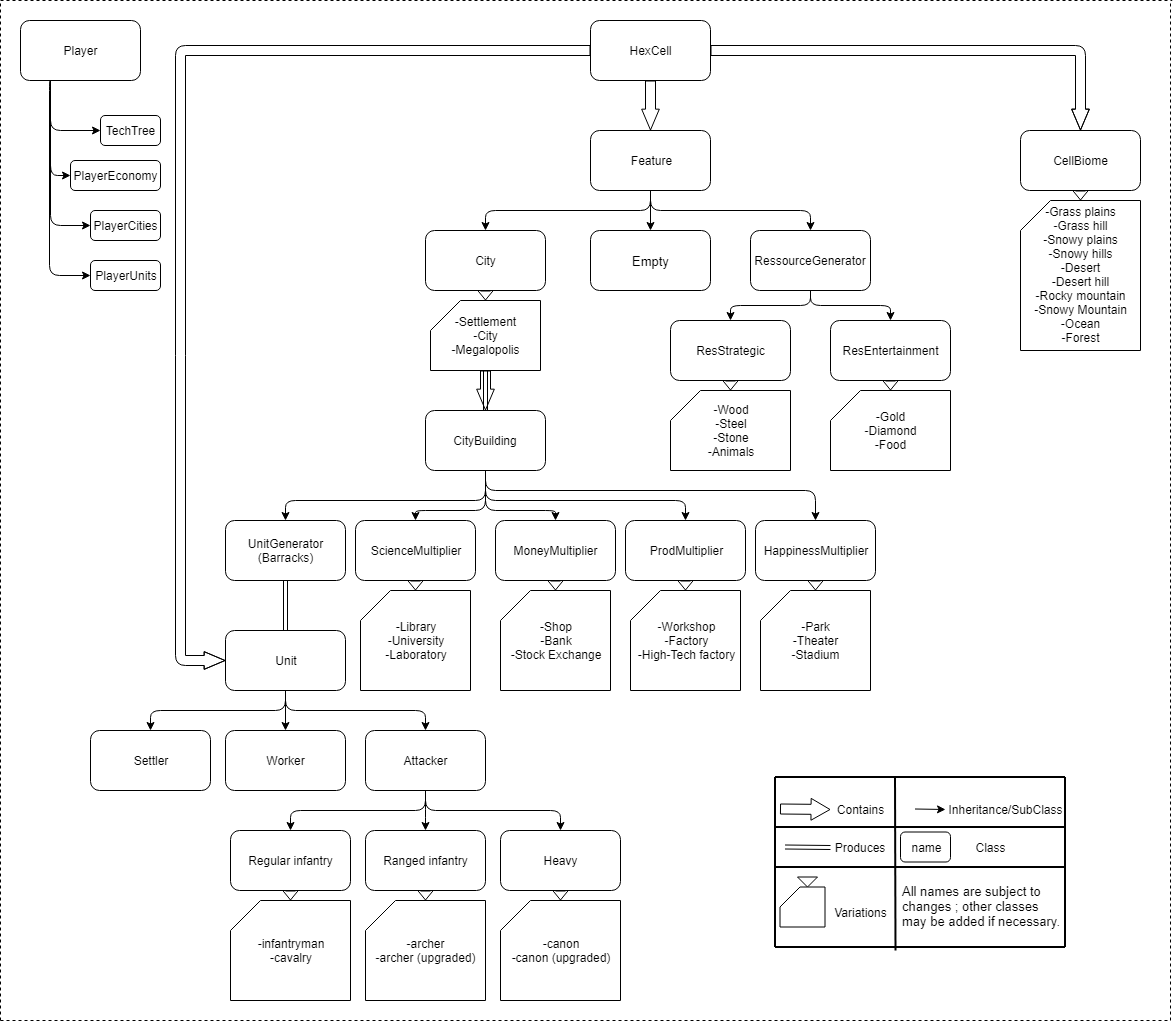
\includegraphics[width=1\textwidth]{../report_1/img/class_hierarchy}
    \caption*{Hiérarchie des classes}
\end{figure}

\subsection{Joueurs}

La classe Player est une classe majeure pour le bon déroulement d’une partie.
C’est la classe qui est directement lié au joueur et qui va contenir toutes les
informations qui lui sont propres. Ces informations sont notamment:

\begin{itemize}
    \item Un lien vers chaque ville et chaque unité que le joueur possède,
        possédant tous un identifiant unique
    \item Les quantités de chaque ressource possédées par le joueur
    \item L’état du joueur (en jeu, spectateur, vainqueur)
\end{itemize}

Cette classe permet aussi de faire le lien entre les différents systèmes,
notamment la création et l’attribution de villes et d’unités, mais aussi le lien
avec le réseau, et les éléments de sécurité pour éviter qu’un joueur ne puisse
former ou déplacer des troupes sans limite par tour.

\subsection{Unités}

Les unités sont réparties en plusieurs catégories, chacune avec un but précis et
des caractéristiques adaptées. Les unités à but offensif possèdent également une
version évoluée au niveau 11 (avec des caractéristiques améliorées et une
apparence différente) et ont la possibilité de gagner des niveaux, de 1 à 20,
durant la partie (chaque niveau augmente leur attaque et leurs points de vie).
Voici les unités présentes dans le jeu:

\subsubsection{Le colon (unité pacifique)}

Le colon est une unité extrêmement importante. Elle permet de fonder une ville,
et donc joue un rôle crucial dans l’expansion de l’empire du joueur. Toutefois,
afin de la rendre équilibrée, c’est aussi une unité qui nécessite beaucoup de
ressources, et qui peut être éliminée très facilement (ne possédant pas
d’amélioration, elle possède le même nombre de points de vie, peu importe la
progression du joueur, là où les unités d’attaque deviennent plus puissantes).

\subsubsection{L'ouvrier (unité pacifique)}

Le travailleur est une unité indispensable au joueur, car c’est elle qui permet
d’exploiter les différentes ressources de la map. Les ressources stratégiques et
de luxe sont indispensables au fonctionnement interne de l’empire, tant pour les
unités, que l'économie ainsi que pour la population. Autrement dit, sans
travailleur, la durée de vie du joueur sera très limitée. Il s’agit donc d’une
unité peu coûteuse à former, mais tout de même relativement fragile. De plus, à
l’instar du colon, cette unité n’est pas améliorable.

\subsubsection{Le fantassin (unité offensive standard)}

Le fantassin est l’unité offensive par défaut. Ses caractéristiques de combat ne
sont pas les plus puissantes. Son intérêt peut alors sembler limité, mais pour
compenser ces caractéristiques qui ne sortent pas de l’ordinaire, le fantassin
reste également une unité peu coûteuse, et peut ainsi être recruté assez tôt
dans la partie sans mettre le joueur en difficulté au niveau des ressources. Le
fantassin, une fois amélioré, devient un cavalier, qui dispose d’une vitesse de
déplacement accrue, faisant ainsi de cette unité “standard” l’unité de choix
pour l’exploration et les offensives rapides, ou pour réagir rapidement à une
invasion ennemie. Cette unité est aussi la plus efficace contre les unités
lourdes.

\subsubsection{L'archer (unité offensive longue portée)}

L’archer est une unité offensive spécialisée dans l’attaque d’autres unités
humaines, mais extrêmement désavantagée face aux unités lourdes et aux villes.
La caractéristique principale de l’archer est sa portée d’attaque qui lui permet
d’être le premier à attaquer, et de rester hors d’atteinte d’une contre-attaque
ennemie. En revanche, l’archer est la plus fragile des unités offensives, ce qui
signifie que sa puissance importante contre les autres unités perd tout son
intérêt en combat rapproché ou en infériorité numérique, où l’ennemi pourra
riposter. L’archer, dans sa forme améliorée, gagne en puissance, ce qui accentue
davantage sa fonction de “chasseur de troupes”.

\subsubsection{La catapulte (unité offensive lourde)}

La catapulte est une unité très spéciale. Plus lente que les autres, mais très
résistante face aux archers, elle brille notamment contre les villes et
ressources ennemies. C’est évidemment l’unité la plus dangereuse du jeu, car
elle permet de détruire une cité adversaire en seulement deux à cinq tours, là
où un soldat prendrait plus de deux fois cette durée. Pour équilibrer cela, la
catapulte a un coût de production très onéreux, proche de celui du colon, et
sera bien moins efficace contre les autres unités offensives. Il faut donc
toujours veiller à l’accompagner d’autres troupes pour la défendre. La
catapulte, une fois améliorée, devient un canon. Sa puissance de destruction
contre les villes est alors augmenté, ainsi que sa portée, la rendant plus
dangereuse que jamais, et en faisant donc une cible prioritaire, car élément clé
à la victoire.

La notion de stratégie est donc très présente dans le jeu. Le joueur va devoir
apprendre à gérer les différentes unités, leurs améliorations, les ressources,
et s’adapter au jeu. Il est impossible de gagner la partie en se contentant d’un
unique type d’unité produite en masse, car chacune possède des points faibles
facilement exploitables par l’adversaire.

\subsection{Villes}

Les villes représentent la base de l’empire du joueur: sans ville, il lui est
impossible de former de nouvelles unités ou de récolter de ressources. Une fois
que toutes les villes d’un joueur sont détruites, il ne lui restera en général
que peu de tours de survie avant que toutes ses unitées restantes ne soient à
leur tour détruite, terminant ainsi sa partie.

Chaque ville possède trois niveaux, et évolue d’elle même en fonction du nombre
d’habitant. Chaque niveau débloque de nouvelles unités et de nouveaux bâtiments
pour cette ville :

\begin{itemize}
    \item Colonie (à partir de 0 habitant) : Le statut de base, permet de
        construire les bâtiments de rang 1, ainsi que la formation du
        travailleur et du fantassin.
    \item Ville (à partir de 1 000 habitants) : Débloque la construction des
        bâtiments de rang 2, et la formation du colon et de l’archer.
    \item Mégapole (à partir de 5 000 habitants) : Permet de construire des
        bâtiments de rang 3, et de former des catapultes
\end{itemize}

Notez que, à l’inverse des unités qui possèdent un niveau global lié au joueur,
chaque ville possède son propre avancement. Ainsi vous ne pouvez pas fonder une
nouvelle ville près de l’adversaire et directement commencer à entraîner des
unités lourdes. La population augmente petit à petit à chaque tour, mais sa
croissance peut être favorisée par des bâtiments dans les villes. Ces bâtiments,
qui ne sont pas représentés visuellement, donnent des bonus dans les domaines
suivant:

\begin{itemize}
    \item Science : augmente le niveau des troupes, il s’agit d’une ressource
        globale liée au joueur.
    \item Monnaie : permet d’acheter des unités dans une ville du joueur.
    \item Production : influe sur la vitesse de formation d’unités ou de
        création de bâtiments. Chaque ville a son propre niveau de production.
    \item Joie : influe sur la croissance de la population. Une joie trop faible
        conduira à des malus pour les domaines précédents. Il s’agit d’une
        valeur propre à chaque ville.
\end{itemize}

Ces quatre domaines sont en lien direct avec le nombre d’habitants. Il est donc
intéressant de continuer de développer une ville après avoir atteint le statut
de mégapole, même si cela devient plus négligeable.

\subsection{Économie}

L’économie ne s’arrête pas qu’aux quelques éléments vus ci-dessus. En effet, il
existe encore des ressources disponibles sur la carte, divisées en deux groupes
: ressources stratégiques (qui permettent de produire ou améliorer des unités),
et ressources de luxe (qui permettent de construire les bâtiments liés à la
joie).

\begin{itemize}
    \item Bois (stratégique)
    \item Chevaux (stratégique)
    \item Fer (stratégique)
    \item Or (de luxe)
    \item Diamant (de luxe)
    \item Nourriture (de luxe)
\end{itemize}

Elles sont toutes spécifiques au joueur et peuvent être obtenues en exploitant
des cases grâce aux travailleurs. Une certaine quantité de ressource est alors
produite à chaque tour sur ces cases. Attention toutefois car ces exploitations
sont des structures pouvant être détruites.

Il est donc important de posséder le plus d’exploitations possible. En effet, un
plus grand nombre implique une plus grande quantité de ressources produites à
chaque tour, et ainsi un développement plus rapide. De plus, ces ressources
n’ont pas de limites de stockage, ce qui signifie que faire des réserves
représente un avantage en cas d’attaque adversaire.

\subsection{Biomes}

Un dernier élément du gameplay qui semblait important pour ce type de jeu était
l’impact des différents types de terrain sur les unités. En effet, chaque biome
a un effet sur le déplacement des unités, leurs vitesses, ainsi que leurs
portées de vue. Cela a pour but de favoriser certains chemins selon l’action
souhaitée : une attaque rapide via une plaine, camouflée via une forêt, ou
encore l'exploration à l’aide de la hauteur d’une montagne.

\section{IA (Thibault)}

\subsection{Fonctionnement}

L’intelligence artificielle du mode solo est constituée de plusieurs
composantes. Des unités barbares vont apparaître sur la carte, proche des villes
du joueur afin de tenter des invasions plus ou moins régulières. De plus, un
système de malus du développement interne du joueur permet d’ajouter une part de
difficulté. La force des unités, leurs nombres, leurs taux d’apparition, la
difficulté de l’économie/production, et d’autres caractéristiques de l’IA sont
régulées par un niveau de difficulté choisi par le joueur en début de partie :

\begin{itemize}
    \item Facile : des unités barbares d'un niveau faible par rapport au joueur
        (entre -3 et -2 niveaux de différence) qui apparaîtront de manière
        individuelle toutes les quinzaines de tours. Aucun malus sur l'empire.
    \item Normal : les barbares ont un niveau semblable ou légèrement plus fort
        que celui du joueur (entre 0 et +1 niveau de différence) et apparaissent
        par groupe de deux environ tous les 13 tours. Chaque aspect de
        développement de l'empire (économie, science, production) recevra un
        malus de -7.5\%.
    \item Difficile : des barbares féroces d'un niveau technologique plus élevé
        (+3 niveaux de différence) débarqueront par binômes environ tous les 10
        tours. Le développement économique et de production reçoivent un malus
        de -12\%, tandis que celui scientifique de -9.
\end{itemize}

\subsection{Construction}

À chaque fois qu’une tribu barbare apparaît (dans un rayon proche d’une ville),
les unités vont se déplacer vers la ville la plus proche encore debout afin de
l’attaquer. Avec le système de pathfinding déjà fonctionnel, il était facile
d’intégrer l’IA au reste du code, qui fera donc office d’un joueur
supplémentaire pour le mode solo.

Pour gérer les malus internes du joueur, nous avions déjà en place un système
permettant de différencier les différents modes de jeu (solo, multi, éditeur de
carte)

\section{Interface (Valérian \& Cédric)}

\subsection{Menu principal}

Notre menu principal à beaucoup évolué au fil du projet. Parti de quelques
boutons ayant pour unique but de tester rapidement les fonctionnalités
implémentées, faisant fi de l’esthétique, nous avons évolués vers une interface
ergonomique, visuellement agréable et pratique. Nous avons utilisé un asset créé
et mis à disposition gratuitement par Michsky. Reprendre un menu existant nous
permettait de nous concentrer sur d’autres aspects graphiques du jeu nécessitant
une réelle customisation pour suivre le thème de Pacification comme l’interface
de jeu ou les modèles 3D des unités.

Nous avons toutefois personnalisé cet asset afin de le faire rentrer dans
l'ambiance du jeu. Le menu principal se compose de 4 boutons majeurs :

\begin{itemize}
    \item Bouton Play : permet de lancer une partie en solo ou en multijoueur
    \item Bouton Editor : démarre l'éditeur de carte
    \item Bouton Settings : accède aux paramètres du jeu comme le volume, la
        langue ou encore la luminosité
    \item Bouton Exit : quitte le jeu
\end{itemize}

La naviguation entre les menus se fait grâce à des déplacements de caméras sur
différents canvas, ainsi que de boutons pour revenir en arrière sur chaque
panel.

\subsubsection{Lobbys de jeu}

Au démarrage de chaque partie solo, un menu permet au joueur de définir les
options de génération de la carte en fonction de ce qu’il souhaite, ou de
charger une map déjà préparée et sauvegardée sur son ordinateur.

En ce qui concerne les parties multijoueur, chaque joueur voit un premier menu
où il renseigne son speudo, ainsi que l'IP du serveur. Après connexion, les
clients passent sur un second menu listant les différents joueurs actuellement
connectés. L'hôte de la partie décidera des options de génération de la carte,
ou encore de charger une sauvegarde depuis un fichier.

\subsubsection{Contrôles}

Dans les options du menu principal, il est possible d’afficher et de modifier
les différents contrôles du jeu : son, langue, luminosité, etc

\subsection{Interface de jeu}

En ce qui concerne les interfaces dans le jeu, nous sommes restés simple sur le
design, parce que beaucoup de complexité était déjà présente au niveau de la
gestion de chaque panel pour conserver une bonne ergonomie.

Sélectionner une unité ou une construction dans le jeu fait apparaître un menu
correspondant à cette object. Une selection de ville fera par exemple apparaître
l’interface de la caserne permettant de développer des unités. Dans les menus de
chaque objet apparaît aussi sa vie restante, son appartenance (quel joueur
détient cet objet) et quelques statistiques à son sujet.

En jeu comme en mode éditeur un bandeau d’information est disponible en haut de
l’écran. Il affiche en jeu des informations sur le joueur et son empire (argent,
productivité, science, bonheur de la population) ainsi que le nombre de tours
qui est passé et un accès au menu pour se déconnecter.

Enfin, un tchat est disponible pour s’envoyer des messages ou utiliser des
commandes spéciales. Son développement a représenté un certain challenge vis à
vis de l’interface, mais aussi du déroulement du jeu, pour que son utilisation
n’interfère pas avec le jeu même, mais représente un élément important notamment
pour l’aspect multijoueur.

\subsection{Éditeur}

L’interface de l’éditeur de map reste simple et se compose d’un bandeau qui
contient des boutons permettants de sauvegarder, charger ou générer une carte
facilement et rapidement.

Sur les bords droit et gauche de l’écran, des panels permettent de changer ce
qui sera modifier le terrain (biome, eau, élévation) mais aussi ce qui est
présent sur ce terrain comme les ressources inexploitées (minerais, forêts,
champs, …) 

\section{Site web (Valérian)}

\subsection{Développement}

En ce qui concerne le développement du site, celui ci est composé d’HTML, de CSS
ainsi que de PHP.

Pensé pour être pratique au niveau de la navigation, le site reste simple dans
son design, et clair, en ne surchargeant pas le visiteur d’informations. 

Son développement s’est déroulé sans accrocs et en avance sur le planning
défini.

\subsection{Hébergement}

Si dans un premier temps notre site était hébergé grâce à GitPages, il à été
nécessaire de changer d’hébergement à mesure que son développement avançait. En
effet, avec l’arrivée de PHP dans le site, il était impossible de rester sur
notre premier choix d'hébergement qui ne le supportait pas.

Nous avons donc migré le site vers un hébergement fourni par Lixia, un groupe
qui propose beaucoup de services de ce type gratuitement.

Cela nous a permis d’obtenir un nom de domaine \url{pacification.lxa.li}, ainsi
que des adresses mails pour proposer un support technique du jeu. 

\subsection{Fonctionnalités}

Notre site web se compose de 6 onglets permettant d'accéder à toutes les
informations pour suivre le développement.

L’onglet “Accueil” permet de suivre l’avancée du jeu grâce à un listing des
mises à jour et un détail de ce qui à été ajouté.

L’onglet “Comment jouer ?” permet aux joueurs d’apprendre à prendre en main
notre jeu, en détaillant le déroulement d’une partie et quelques stratégies pour
bien commencer.

L’onglet “L’équipe” présente les membres de l’équipe qui à développé ce jeu, en
offrant quelques anecdotes sur eux.

L’onglet “Ressource” donne crédits aux différents éléments de créateurs que nous
avons pu utiliser dans le développement du jeu, tel que les musiques, ou l’asset
du menu.

L’onglet “Contenu supplémentaire” offre quant à lui la possibilité aux joueurs
de télécharger et/ou proposer des maps de jeu créé dans l’éditeur du jeu. Cela
permet de proposer une dimension de jouabilité plus grande avec donc la
possibilité de créer des scénarios de jeux et les partager avec la communauté de
joueurs.

L’onglet “Téléchargement” permet pour sa part de télécharger la dernière version
du jeu.

Egalement disponible sur toutes les pages, sont présentes les archives de notre
développement, comprenant les version du jeu à chaque soutenance, ainsi que les
divers documents à rendre tel que le cahier des charges et les rapports de
soutenances.

Diverses images et captures du jeu sont disponibles sur le site afin de
permettre aux visiteurs d’avoir une idée de celui-ci.

\section{Assets (Cédric)}

\subsection{Design}

Pour l’aspect général du jeu nous avons opté pour un style cartoon low poly afin
d’obtenir un rendu visuel agréable mais également pour éviter que les modèles ne
soient trop complexes à créer.

\subsection{Création}

Créer les objets 3D se déroule en plusieurs étapes et les méthodes ont été
différentes en fonction du type d’objet à concevoir. Pour les unités, il fallait
un modèle original sur lequel se baser afin de faire toutes les unités humaines.
Pour sa conception, un dessin est utilisé comme référence, puis différentes
modifications sont appliquées à un cube (extrusion, rotation, élargissement,...)
afin de faire correspondre la forme que créé à partir avec le dessin. Blender
possède des options fortement utiles comme l’option miroir qui permet de n’avoir
qu’à créer qu’un seul côté d’un objet tandis que l’autre se crée automatiquement
par symétrie. Une fois le personnage créé, une autre fonctionnalité de Blender
appelée “subdivision surface” permet de diviser les polygones constituant le
personnage en d’autres plus petits, permettant ainsi d’arrondir les parties
visuelles trop angulaires et disgracieuses du modèle. Une fois ce modèle
humanoïde créé, pour fabriquer les morceaux d’armures et et de vêtements, il a
suffit d’extruder et d’élargir certaines parties et de séparer des morceaux de
l’objet afin de pouvoir leur attribuer à chacun une texture différente. Les
armes ont quant à elles été conçu en se basant sur des images, de la même
manière que le modèle humain.

Concernant les différents bâtiments, il a fallu créer les différentes parties
(piliers de bois, toit, rempart et tour du château,...), ensuite les assembler
de diverse manière pour obtenir différentes formes tout en gardant un aspect
esthétique cohérent. Le procédé fut le même pour l’environnement naturel des
bâtiments de ressources : De nombreuses formes de rochers et d’arbres ont été
fabriqués puis dupliqués afin de créer les mines et les forêts.

Toutes les textures ont été créées par notre équipe grâce aux fonctionnalités
proposé par Blender et au logiciel de dessin Krita. Pour les appliquer sur les
modèles 3D, nous utilisons une méthode appelée “UV Mapping”. Il faut pour cela
“découper” notre objet 3D afin d’obtenir l’équivalent d’un patron qui sera
déplacé et modifié sur l’image qui servira de texture à l’objet. Pour d’autres
parties commes les armures des unités nous n’avons pas utilisé cette technique
et nous nous sommes contenté de créer un nouveau matériau en lui donnant une
couleur spécifique et en modifiant certaines propriétés pour qu’il reflète la
lumière plus ou moins bien.

Une fois les modèles créés, ils sont importés sur Unity. Pour cela il a fallu
exporter les modèles 3D sous le format FBX avec les matériaux et les textures
utilisés. Il suffit alors ensuite d’assigner les bonnes textures aux bons
matériaux et les bons matériaux aux modèles 3D.

Les textures utilisées pour les différents biomes présents sur la carte du jeu
ont été créées de manière procédurale grâce à un plug-in de Unity appelé “Number
Flow”.

\subsection{Animations}

Pour animer les unités il fallait tout d’abord des armatures. Un premier
squelette avait été construit sur le modèle humanoïde de référence cependant,
l’animation manuelle des différentes parties du corps étaient extrêmement
difficile à maîtriser et le résultat obtenu était très loin d’être convenable.
Par conséquent pour les unités humanoïdes, nous avons exporté nos unités sur le
site Mixamo qui permet de créer une armature automatiquement sur nos personnages
en se basant sur des points de repères (menton, coudes, genoux,...) que nous
plaçons sur eux. De plus le site possède une bibliothèque très complète de
diverses animations de personnages. Nous avons donc utilisé des animations
adaptés à nos unités comme pour les soldats d’infanterie pour lesquels nous
avons choisi des animations de personnages maniant l’épée et le bouclier.

Cependant ce site ne s’occupe que des modèles humanoïdes. Pour animer d’autres
unités comme la catapulte il a fallu recourir aux armatures créées dans blender.
Pour ce modèle cela ne fut pas très compliqué car les différents os n’étaient
pas relié entre eux.  Un os pour bouger le “bras” de la catapulte, et 4 os pour
faire tourner les roues. Pour créer l’animation il faut utiliser l’armature pour
faire bouger le modèle 3D et enregistrer les positions de l’objet pour une
image. Par exemple en enregistrant les positions du “bras” de la catapulte à sa
position de base à l’image 0 puis à l’image 10, Blender va créer lui même
l’animation grâce aux positions de références.

Pour les unités il y a 3 types d’animations : Une d’attaque, une de déplacement
et une animation de mort.

\subsection{Son}

Différentes musiques se lancent pendant le déroulement du jeu, permettant
d’ajouter une ambiance sonore agréable favorisant l’immersion du joueur.

Plusieurs effets sonores sont aussi présents comme la notification de message
dans le tchat, ou l’apparition d’une tribu barbare dans les environs.

\section{Logos (Valérian)}

\subsection{Création}

En ce qui concerne le logo PACIFICATION, il a été réalisé en se basant sur une
police d’écriture nommée Cubix, qui a ensuite été modifiée par nos soins sur le
site FontStruct.

Le logo de Brainless Devs’, nom de notre groupe, à été plus complexe à réaliser.
Il a fallu dans un premier temps définir tous ensemble le caractère de notre
logo, avant de se lancer dans sa construction. Nous sommes parti vers quelque
chose de simple et clair, en noir et blanc.

Souhaitant avoir autre chose que du texte dans ce logo, nous avons représenté un
Stickman assis, adossé aux initiales du nom du groupe. Afin qu’il corresponde au
nom, il a été représenté avec un ordinateur sur les genoux, codant. Sa tête est
quant à elle une bulle vide, évidente référence au “Brainless”.

La réalisation même du logo à été faite par notre équipe à l’aide d’un stylet et
d’une tablette graphique.

\subsection{Inspiration}

L’inspiration du Stickman provient des animations d’Alan Becker, sur Youtube,
qui représente les aventures de Stickmen s’agitant dans un écran d’ordinateur
ainsi que des webcomics xkcd (xkcd.com). 

\chapter{Expériences personnelles}

\section{Thibault}

\section{Valérian}

Au cours des mois qui ont suivi le début du projet,j’ai pu apprendre beaucoup,
et je retire de cette expérience de bon souvenirs. Si dans un premier temps, je
me suis principalement concentré sur le réseau du jeu, et donc du code pur, j’ai
pu ensuite découvrir d’autres aspects du projet en travaillant sur l’interface
de jeu. Cela m’a appris à mieux utiliser et maîtriser Unity. 

C’est aussi avec l’outil de collaboration Git que mon expérience grandit.
L’ayant en effet utilisé pour le développement du projet, j’ai pu en apprendre
plus à son sujet et à sa manipulation. 

C’est au final beaucoup de compétences nouvelle que j’ai pu acquérir durant ces
derniers mois, et c’est avec beaucoup de joie que je conclue ce projet, heureux
et fier d’avoir, avec mon équipe, mené à bien son développement.

\section{Cédric}

Ce projet m’aura appris l’importance du travail de groupe dans de telles
travaux. Ce fut une expérience enrichissante car j’ai pu améliorer mes
compétences sur des logiciels que j’utilisais déjà auparavant comme Blender mais
j’ai aussi pu apprendre à utiliser Unity que je compte bien continuer à
exploiter pour des projets personnels. 

Il y a eu des moments stressants d’autres plus agréables, mais dans l’ensemble
je suis content d’avoir fait ce projet et surtout je suis fier de ce que j’ai pu
accomplir avec mes camarades. Je n’hésiterai certainement pas à refaire un tel
projet si l’occasion se représentait. 

\section{Antoine}

Pour ma part, ce projet a été une expérience très enrichissante. Cela m’a permi
de découvrir et d’apprendre à me servir du moteur de jeu Unity3D, de m'entraîner
davantage avec le langage C\#. Mais cela m’a surtout donné une petite idée du
fonctionnement des projets de groupe, et des difficultés qui y sont liées.

\chapter{Conclusion}

Pour conclure, Pacification est un jeu de stratégie en tour par tour. La
diversité de ses unités, la génération aléatoire de la carte, ses systèmes
complet et sa prise en main facile en font un jeu complexe mais accessible
cependant au experts comme au novices. Il s’agit d’un jeu auquel on peut jouer
et rejouer, seul ou à plusieurs, en se perfectionnant au fil du temps et en
changeant ses stratégies. Sa légèreté le rend même utilisable sur des
ordinateurs à vocation de bureautique. Et son design cartoonesque en fait un jeu
attractif et non-violent visuellement, qui peut alors convenir à des joueurs de
tout âge.  Nous espérons que vous prendrez autant de plaisir à y jouer que nous
en avons pris à le développer.

\begin{figure}
    \centering
    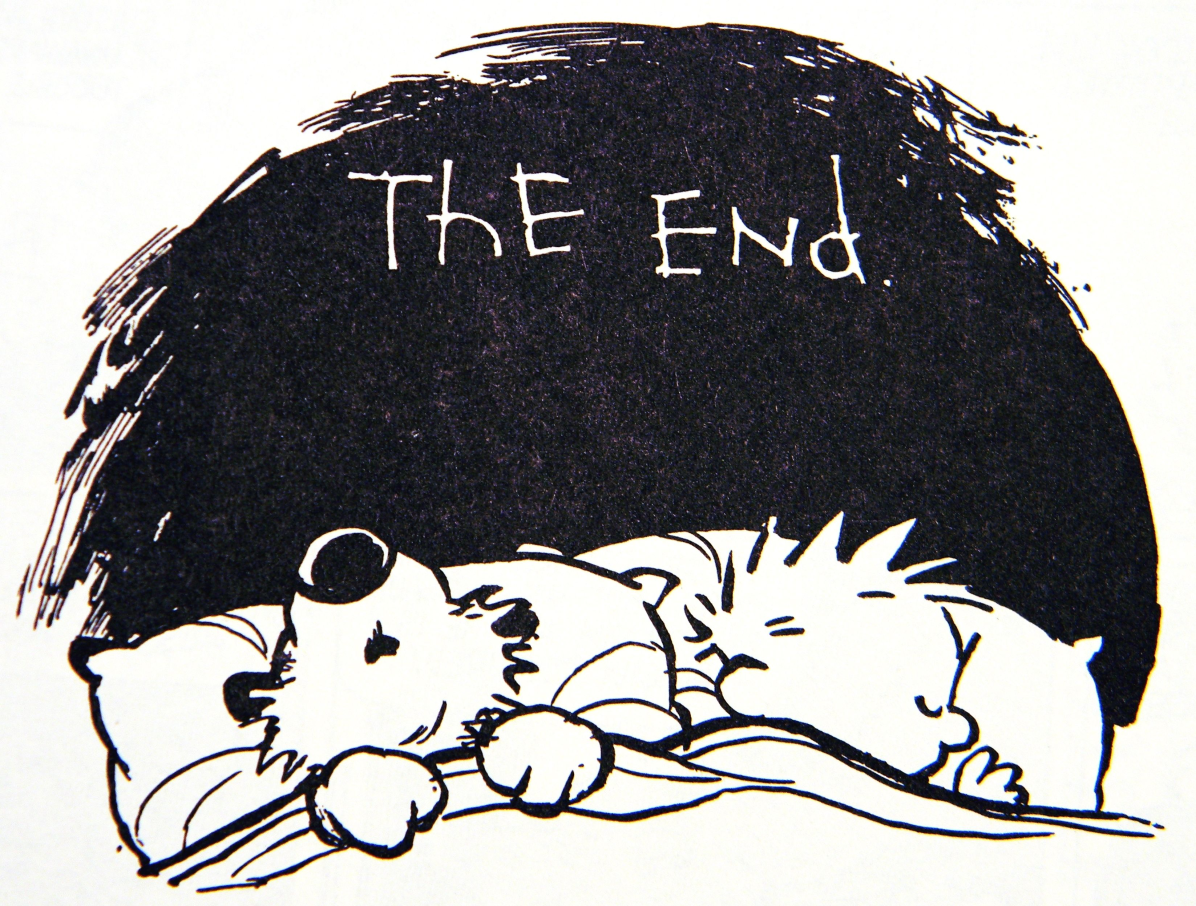
\includegraphics[width=0.8\textwidth]{project_mood}
    \caption*{\textit{Calvin and Hobbes}, Bill Watterson}
\end{figure}

\chapter{Ressources}

Assets 3D
pour le canon
\url{https://www.youtube.com/watch?v=5ivs_jSWraM&t=2050s}

château
\url{https://www.youtube.com/watch?v=HIy1YHC9aes&t=874s}

modèle humanoïde de base
\url{https://www.youtube.com/watch?v=92IdzxwYEWY}

interface du menu principal
\url{https://www.youtube.com/watch?v=nxLc-BaqZag}

Réseau
\url{https://www.youtube.com/watch?v=-nLP0Qz81fE&list=PLLH3mUGkfFCVXrGLRxfhst7pffE9o2SQO}

\end{document}
